\scanpage{6}
\mspage{2.}
word to use else.

\uline{p.19 etc}\margin{!} : I expected lemma 4.3 to be almost trivial but when I tried to write a proof I did not see an easier one\deleted{\unsure{?}}. Also : the proof of lemma 4.4 is kind of subtle (but this could be expected).

p.26. line 1:\quad I shall try to find a precise reference.

line 3 :\quad the condition : irreducible in \uline{Zariski topology} is unpleasant but I have not been able to avoid it.

last line in 3) :\quad it seems necessary to mention also the points $s'$.

p.33,34 etc ..\quad I did not see an easier proof for prop 7.4.

p.43 theor.9.4\quad You have mentioned that the theorem in this form is not satisfactory . for instance the trivial case with constant fib\unsure{re|er}s and arbitrary crossings escapes. However I don't see how to get a satisfactory statement.

p.45. line 5 etc.\quad Is this indication sufficient?

I have not written an appendix on the Lefschetz theory. If you think this is useful then I can still try.
\margin{\figure{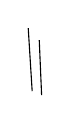
\begin{tikzpicture}\draw (0,0)--(-.05,.8);\draw (.12,-.05)--(.09,.65);\end{tikzpicture}}}

It is not necessary to return the manuscript, I have a carbon copy so you can refer to pages and numbers in your comments. Please give me, if necessary, indications for the way the final manuscript must be typed (is the book a \deleted{foto} photo \unsure{C|c}opy of the manuscript?) Also give me a deadline when you must have the \unsure{M|m}anuscript because I am afraid that I may have already delayed the publication date of your first volume.

With best regards,\\
Sincerely yours,\\
J.P. M\unsure{urre}\\
% archive sheet number: 5
